\chapter{PCB assembly}


\section{SMT lab induction}

You cannot use the SMT lab unless you have performed a lab induction.


\section{Solder pasting}

Solder paste needs to be applied to each pad.  Usually this is applied
using a stencil but for small boards, it can be applied using a
syringe.  The solder paste must be fresh so please return to fridge.


\section{Component placement}

The components are placed onto the pasted pads using a pick-and-place
machine.  The key is to get the orientation of chips, diodes, and LEDs
correct.

It is easy to orient the MCU incorrectly.  The big dot \textbf{does
  not mark pin 1}\footnote{I think they add this to sell more
  chips\ldots}, see \reffig{pin1}.


\begin{figure}[!h]
  \centering
  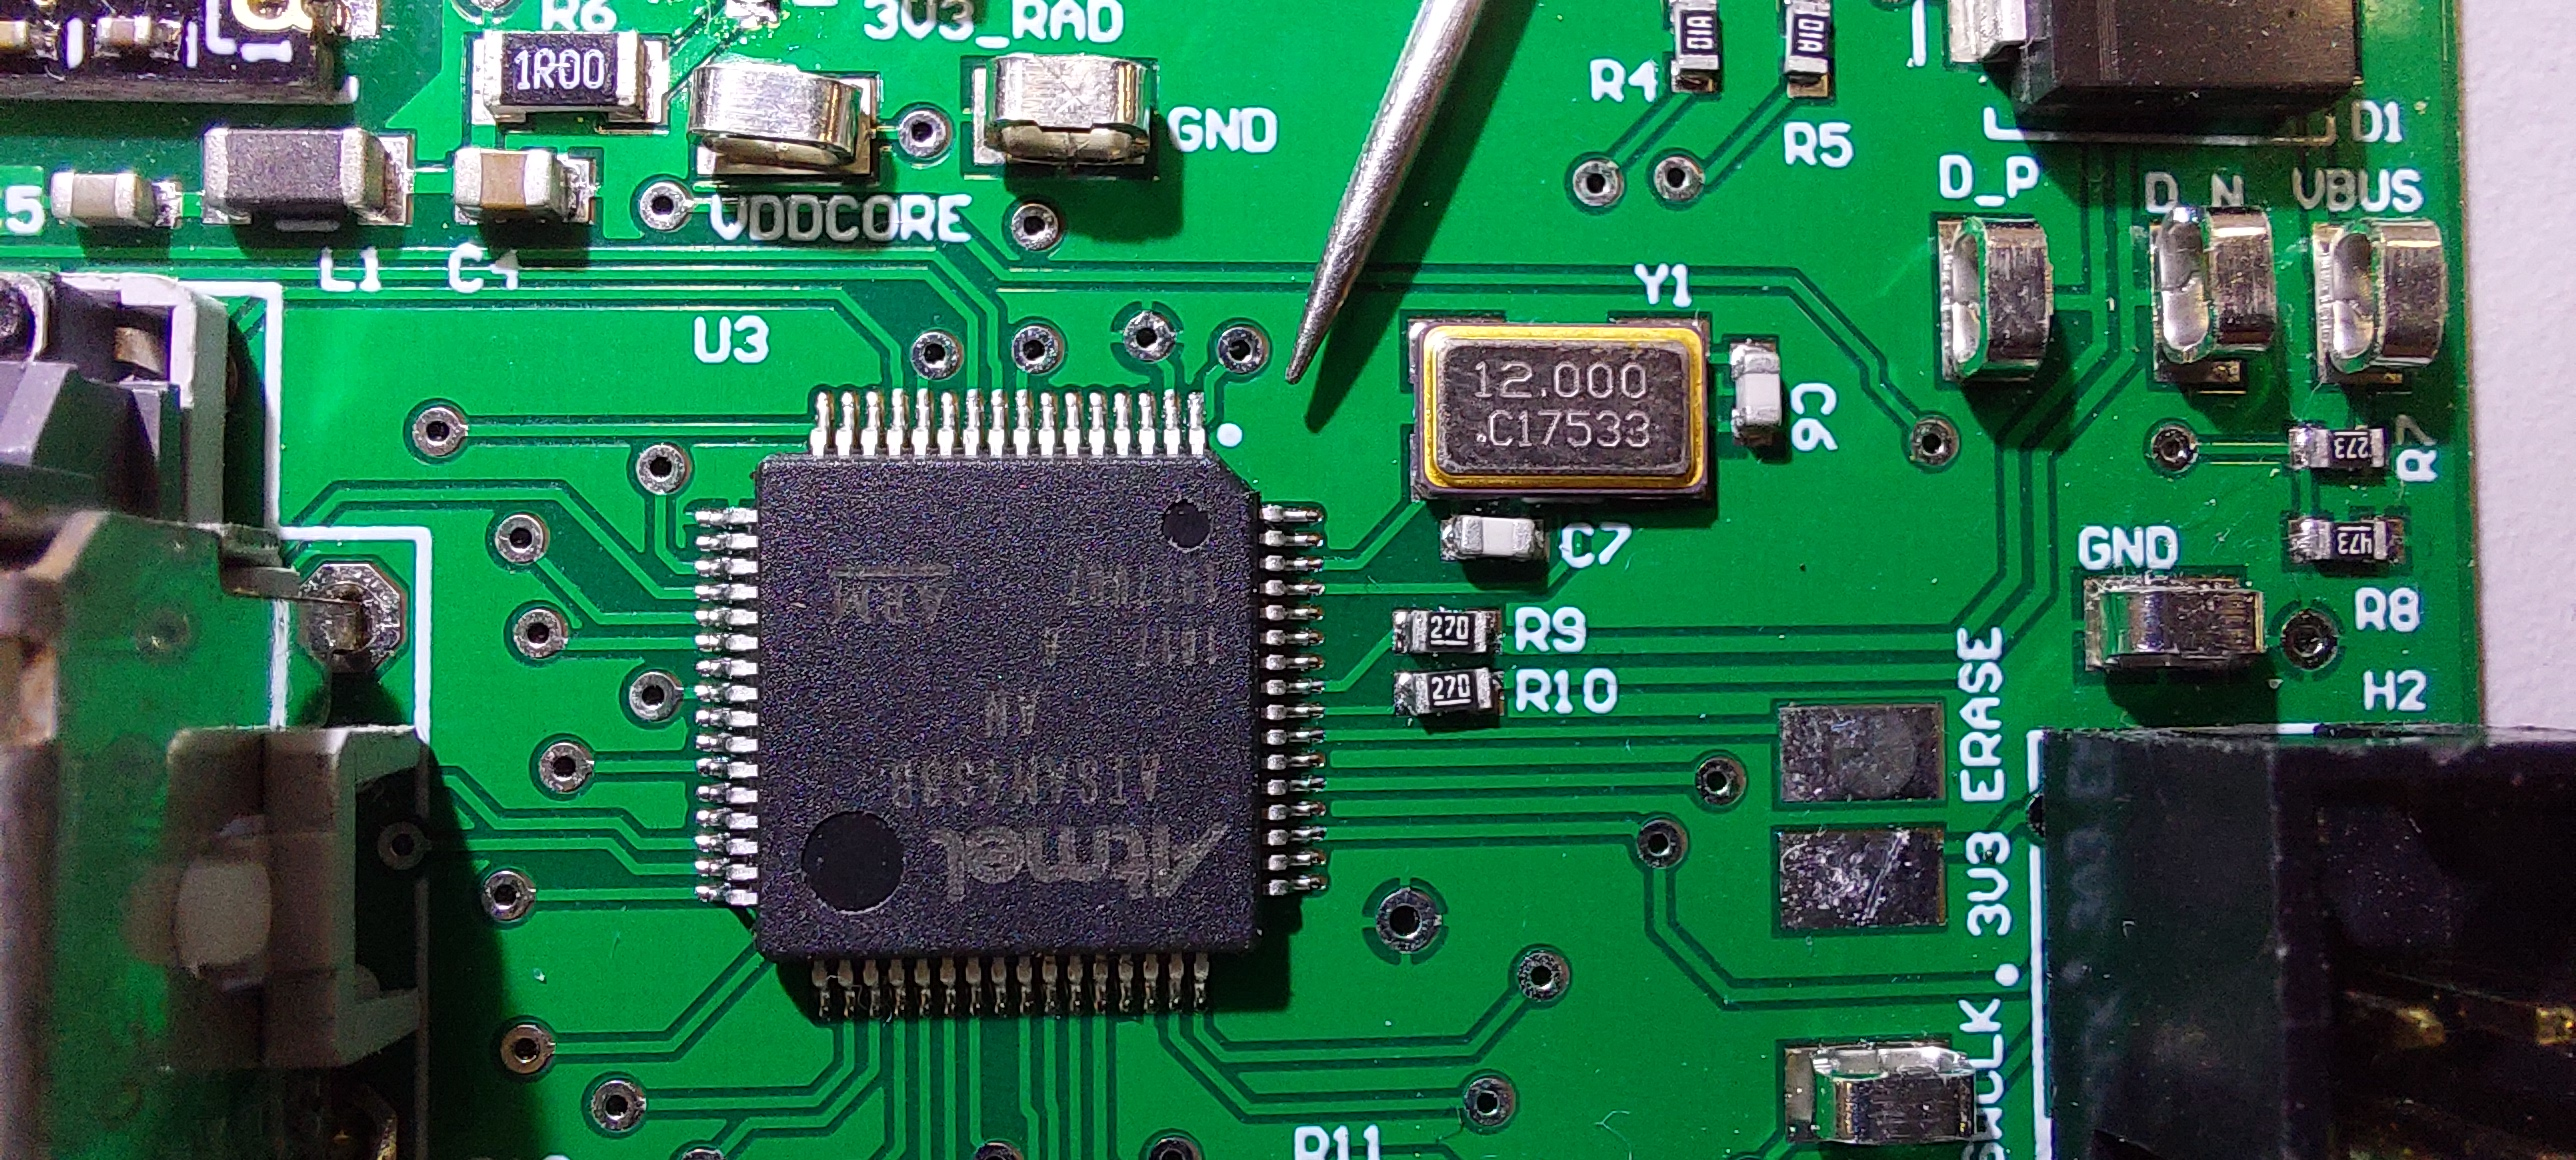
\includegraphics[width=6in]{figs/sam4s_orientation.jpg}
  \caption{Pin 1 of the SAM4S is marked by the chamfer and the small
    dot.}
  \label{fig:pin1}
\end{figure}


\section{Reflow oven}

When the board has been populated, the PCB is placed in the reflow
oven.  Thus is preheated to 150$^{\circ}$ C so you must use oven gloves to
put your board in the oven.  At the end of the process, remove your
PCB using oven gloves.  You do not need to clean the board.


\section{Visual inspection}

Look for solder bridges, see \reffig{solder-bridge}, especially
between IC pins.  The bridges can be removed with a fine-tipped
soldering iron.

\begin{figure}[!h]
  \centering
  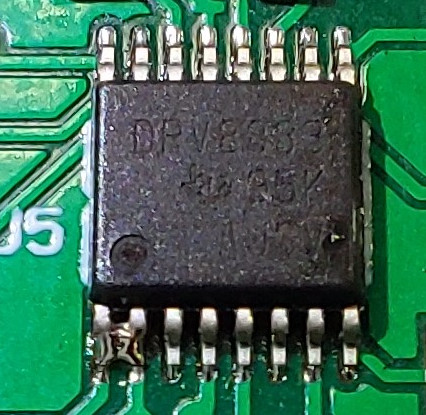
\includegraphics[width=3in]{figs/solder_bridge_zoom.jpg}
  \caption{A solder bridge shorting pins 1 and 2 of the H-bridge.
    This can easily occur if there is too much solder paste.}
  \label{fig:solder-bridge}
\end{figure}
